\documentclass{article}

\usepackage{graphicx}
\usepackage{hyperref}

\begin{document}

\begin{titlepage}
    \centering
    \vspace*{3cm}
    
    
\includegraphics[width=0.4\textwidth]{images/fontyslogo.png} % Adjust the size of the logo
    \vspace{1.5cm}
    
    {\Huge\bfseries Personal Development Report}\\[1cm]
    {\LARGE Evaluation 1}\\[2cm]
    
    \textbf{Danil Burov}\\
    \vspace{0.5cm}
    \textit{Fontys University of Applied Sciences}\\[3cm]
    \vfill
    \textbf{\today}

\end{titlepage}
\newpage
\tableofcontents
\newpage

\section{Introduction}
My name is Danil Burov and I am studying Information Technology in Fontys, Venlo. I am specializing in 
Embedded Software back in Venlo and the reason I chose this minor is because I think that AI is a very 
ongoing topic and I wanted to get more familiar with it. Especially because I think that AI has a big 
implication when it comes down to IoT devices.

\section{Learning outcome 1 - Societal impact}
\underline{\textbf{Description}}\\
The student is able to approach the context and impact of their own AI project(s) 
from different perspectives in a sustainable way. In addition, the student is able to 
reflect on their own choices, taking into account data legislation and the (possible) impact on society.\\\\
\underline{\textbf{Explanation:}}\\
Societal impact is one of the most important contextual parts of the project. Every time a person 
starts a project an evaluation on the societal impact should be done in order to understand 'Why?'
a project is being done on the given topic.
  %Describe the learning outcome how you understand it
\subsection{First evaluation}
During the first weeks of the minor I had the opportunity to think about the societal impact of the projects I will 
be working on. Since the beginning I had an idea of what my personal project could look like. However, I was not that aware
what could be the societal impact of my project. With the help of the technical coach 'Jacco'.\\\\
To see the feedpulse checkpoint regarding this evaluation go to Figure \ref{fig:appendix_image1}.\\\\
\underline{\textbf{Self assesment: Orientating}}\\\\
\subsection{Second evaluation}\\
\subsection{Third evaluation}\\
\subsection{Final evaluaton}\\

\section{Learning outcome 2 - Investigative problem solving}
\underline{\textbf{Description}}\\
The student is able to critically look at their own AI project(s) from different perspectives, 
recognize problems and come up with appropriate solutions.\\\\ 
\underline{\textbf{Explanation:}}\\
From this learning outcome I will further develop my investigative and problem solving skills regarding 
how AI is used in the project, is it doing as intended and if not how to approach the problem and solve it 
eventually.

\subsection{First evaluation}
During the first weeks I had to tackle several problems. In the beginnig the course was presented with some stakeholders 
who presented to us what issues they have with their companies and what they would like to add to their business. I was given 
the opportunity to think of an idea that solves a business case and so I created a project proposal for one of the companies that visited us. 
The proposal is based on the problem that the company has.\\\\
%The link is not working
To see the full proposal go to this link: \href{https://github.com/BurovDanil/MinorAI/blob/main/Documents/Project%20Proposal/Proposal.md}{project proposal}\\\\
  \underline{\textbf{Self assesment: Orientating}}\\\\
\subsection{Second evaluation}\\
\subsection{Third evaluation}\\
\subsection{Final evaluaton}\\

%Upload the project proposal
%During the first weeks I already had to deal with investagative problem solving. In my personal project I had to deal 
%with the legal aspect of my project. In order to solve the issue I went to talk to one of the legal consultants about 
%how I could tackle the problem. In the end of the discussion we managed to resolve the problem with writing a small 'Disclaimer' 
%for the intended usage of the AI model that will be created. As well as during my first stakeholder meeting with my group we were presented
%with an issue. In order to solve the issue and progress into the project we as a group had to think of a sol

\section{Learning outcome 3 - Data preparation}
\underline{\textbf{Description}}\\
The student is able to collect data and estimate its quality and usability. 
The student is also able to adjust the data if necessary for proper usage in their project(s).\\\\
\underline{\textbf{Explanation:}}\\
In order to create any AI model I will need a good, clean dataset that can be used to properly teach a machine.
To do so I intend to first of all use a reliable source for the set and clean inspect it carefully before using.\\\\
\subsection{First evaluation}
The first thing that was done regarding this learning outcome was to select a dataset suitable for the intended usage of the 
AI model. For the personal project I have selected this \href{https://www.kaggle.com/datasets/asaniczka/ufc-fighters-statistics}{dataset}. I have been working on a cleaned version of this dataset. 
Since this dataset does have some empty fields I tried already cleaning some of the data to prepare it for the upcoming modelling. Regarding the data preparation 
for the project I have already started analyzing the data for the organization we are doing the project for, however it is still in a very early stage.\\\\
\underline{\textbf{Self assesment: Orientating}}\\\\
\subsection{Second evaluation}\\
\subsection{Third evaluation}\\
\subsection{Final evaluaton}\\

\section{Learning outcome 4 - Machine teaching}
\underline{\textbf{Description}}\\
The student is able to use data to train models in a way that fits the intended purpose.
The student is also able to test whether the models have been adequately trained.\\\\
\underline{\textbf{Explanation:}}\\
After making sure that the dataset that will be used to teach a machine is not corrupted, outdated and etc., 
I need to ensure that the machine is doing as intended with the dataset. In order to ensure quality, testing the
machine teaching is ideal.\\\\
\subsection{First evaluation}\\
In the first weeks of the minor I explored a website called 'Teachable Machine' in order to get familiar with the steps of creating an 
AI model. The usage of my model was to recognize cats and dogs. The usage of the model can be seen here \ref{fig:appendix_image2}. Other than using the website 
to get familiar with machine learning I have tried to familiarize myself with different machine learning algorithms, such as Decision Trees, Random Forest, etc.
\subsection{Second evaluation}\\
\subsection{Third evaluation}\\
\subsection{Final evaluaton}\\
\underline{\textbf{Self assesment: Orientating}}
\section{Learning outcome 5 - Data visualisation}
\underline{\textbf{Description}}\\
The student is able to use data to create an interesting, informative and 
compelling story in an (interactive) data visualization product, tailored to the right target group.\\\\ 

\underline{\textbf{Explanation:}}\\
Visualizing data will help further understand the relation between different features. In order to achieve this goal,
every correlations that are found between different features need to be visualized. These images need to be understandable and 
self exlpainatory.
\subsection{First evaluation}\\
I have not yet done anything related with data visualization. I have only educated myself with the provided python tutorials and self learning.
\underline{\textbf{Self assesment: }}
\section{Learning outcome 6 - Reporting}
\underline{\textbf{Description}}\\
The student is able to report in a methodologically sound manner on (the outcome of) 
own AI projects (project proposal, process documentation, reporting of final results, etc.).\\\\
\underline{\textbf{Explanation:}}\\
Make sure that documents are written in time and feedback is used to prove the legitamacy of the given goal. The goal would be considered 
accomplished if all documents are consistent and comprehendable. It is very important that the code documentation is easy
to understand and use.\\\\

It is very important that I document the progress I make in order to keep track of how I have improved during the minor. To do so 
I have created my own personal repository which I already have put all the documents I have written up until now. As well as all the exercises 
I have completed for the past 4 weeks. 
\subsection{First evaluation}\\
%Talk about the PDR, personal challenge, the python notebook and the project proposal, and you could mention github docs 
\underline{\textbf{Self assesment: Beginning}}\\\\
\subsection{Second evaluation}\\
\subsection{Third evaluation}\\
\subsection{Final evaluaton}\\

\section{Learning outcome 7 - Personal Leadership}
\underline{\textbf{Description}}\\
The student shows an entrepreneurial mindset regarding their own AI project(s) and personal development, while being aware
of their own learning capacity and keeping in mind professional ambitions in their future work field.\\\\
\underline{\textbf{Explanation:}}\\
The outcome of this learning goal should be that I manage my time correctly without overloading myself. That means following some kind of a schedule, 
as well as attending lectures to ensure that I stay in track and seeking feedback to make sure I am progressing.
\subsection{First evaluation}\\
Ever since the minor started I have attended all lectures regarding the minor and I have taken some things that will help me further develop my skills in AI modelling. 
I still need to improve on asking more feedback from lectures.
\underline{\textbf{Self assesment: Orientating}}\\\\
\subsection{Second evaluation}\\
\subsection{Third evaluation}\\
\subsection{Final evaluaton}\\

\section{Learning outcome 8 - Personal goal}
\underline{\textbf{Description}}\\
With this learning outcome, the student can set its own goal in relation to their future field of work.
This is always related to your Individual Challenge. Describe this Learning Outcome in your PDR.\\\\
\underline{\textbf{Explanation:}}\\
My personal goal for this minor is to get very familiar with how to create an AI model, be able to analyze large amount of data
and prepare this data for further training a given model. I would like to get more familiar with how the machine learning algorithms work 
and be able to choose the appropriate algorithm for the use case.\\\\
\subsection{First evaluation}\\
In the first 4 weeks I have managed to choose a dataset for my own personal project that fits the needs I have, I have attended all lectures to make 
sure I progress in my knowledge for AI technically and ethically. I have managed to import the dataset and clean it based on a condition.\\\\ 
%Exercises for machine learning, the tutorials for Python
\underline{\textbf{Self assesment: Orientating}}\\\\
\subsection{Second evaluation}\\
\subsection{Third evaluation}\\
\subsection{Final evaluaton}\\\\

\section{Retrospect}\\\\ %ONLY IN FINAL VERSION
\section{Conclusion}\\\\ %ONLY IN FINAL VERSION
\section{Appendix}

\begin{figure}[h]
  \centering
  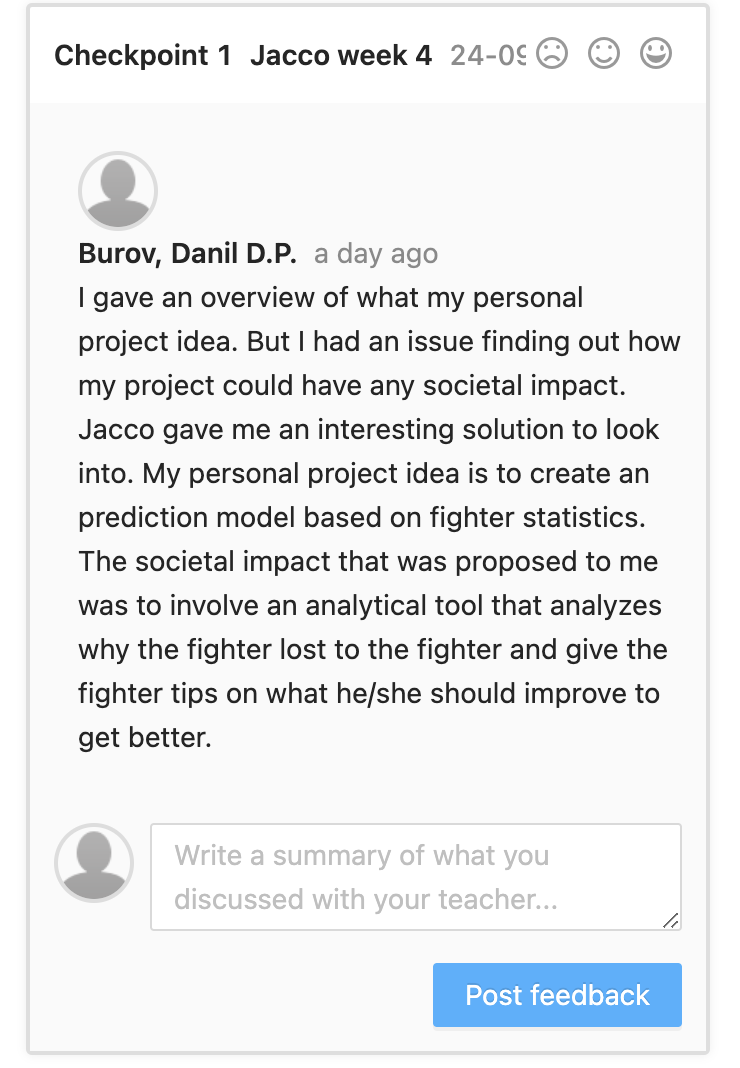
\includegraphics{images/Feedback_Societal_Impact.png}
  \caption{Feedback checkpoint for societal impact}
  \label{fig:appendix_image1}
\end{figure}

\begin{figure}[h]
    \centering
    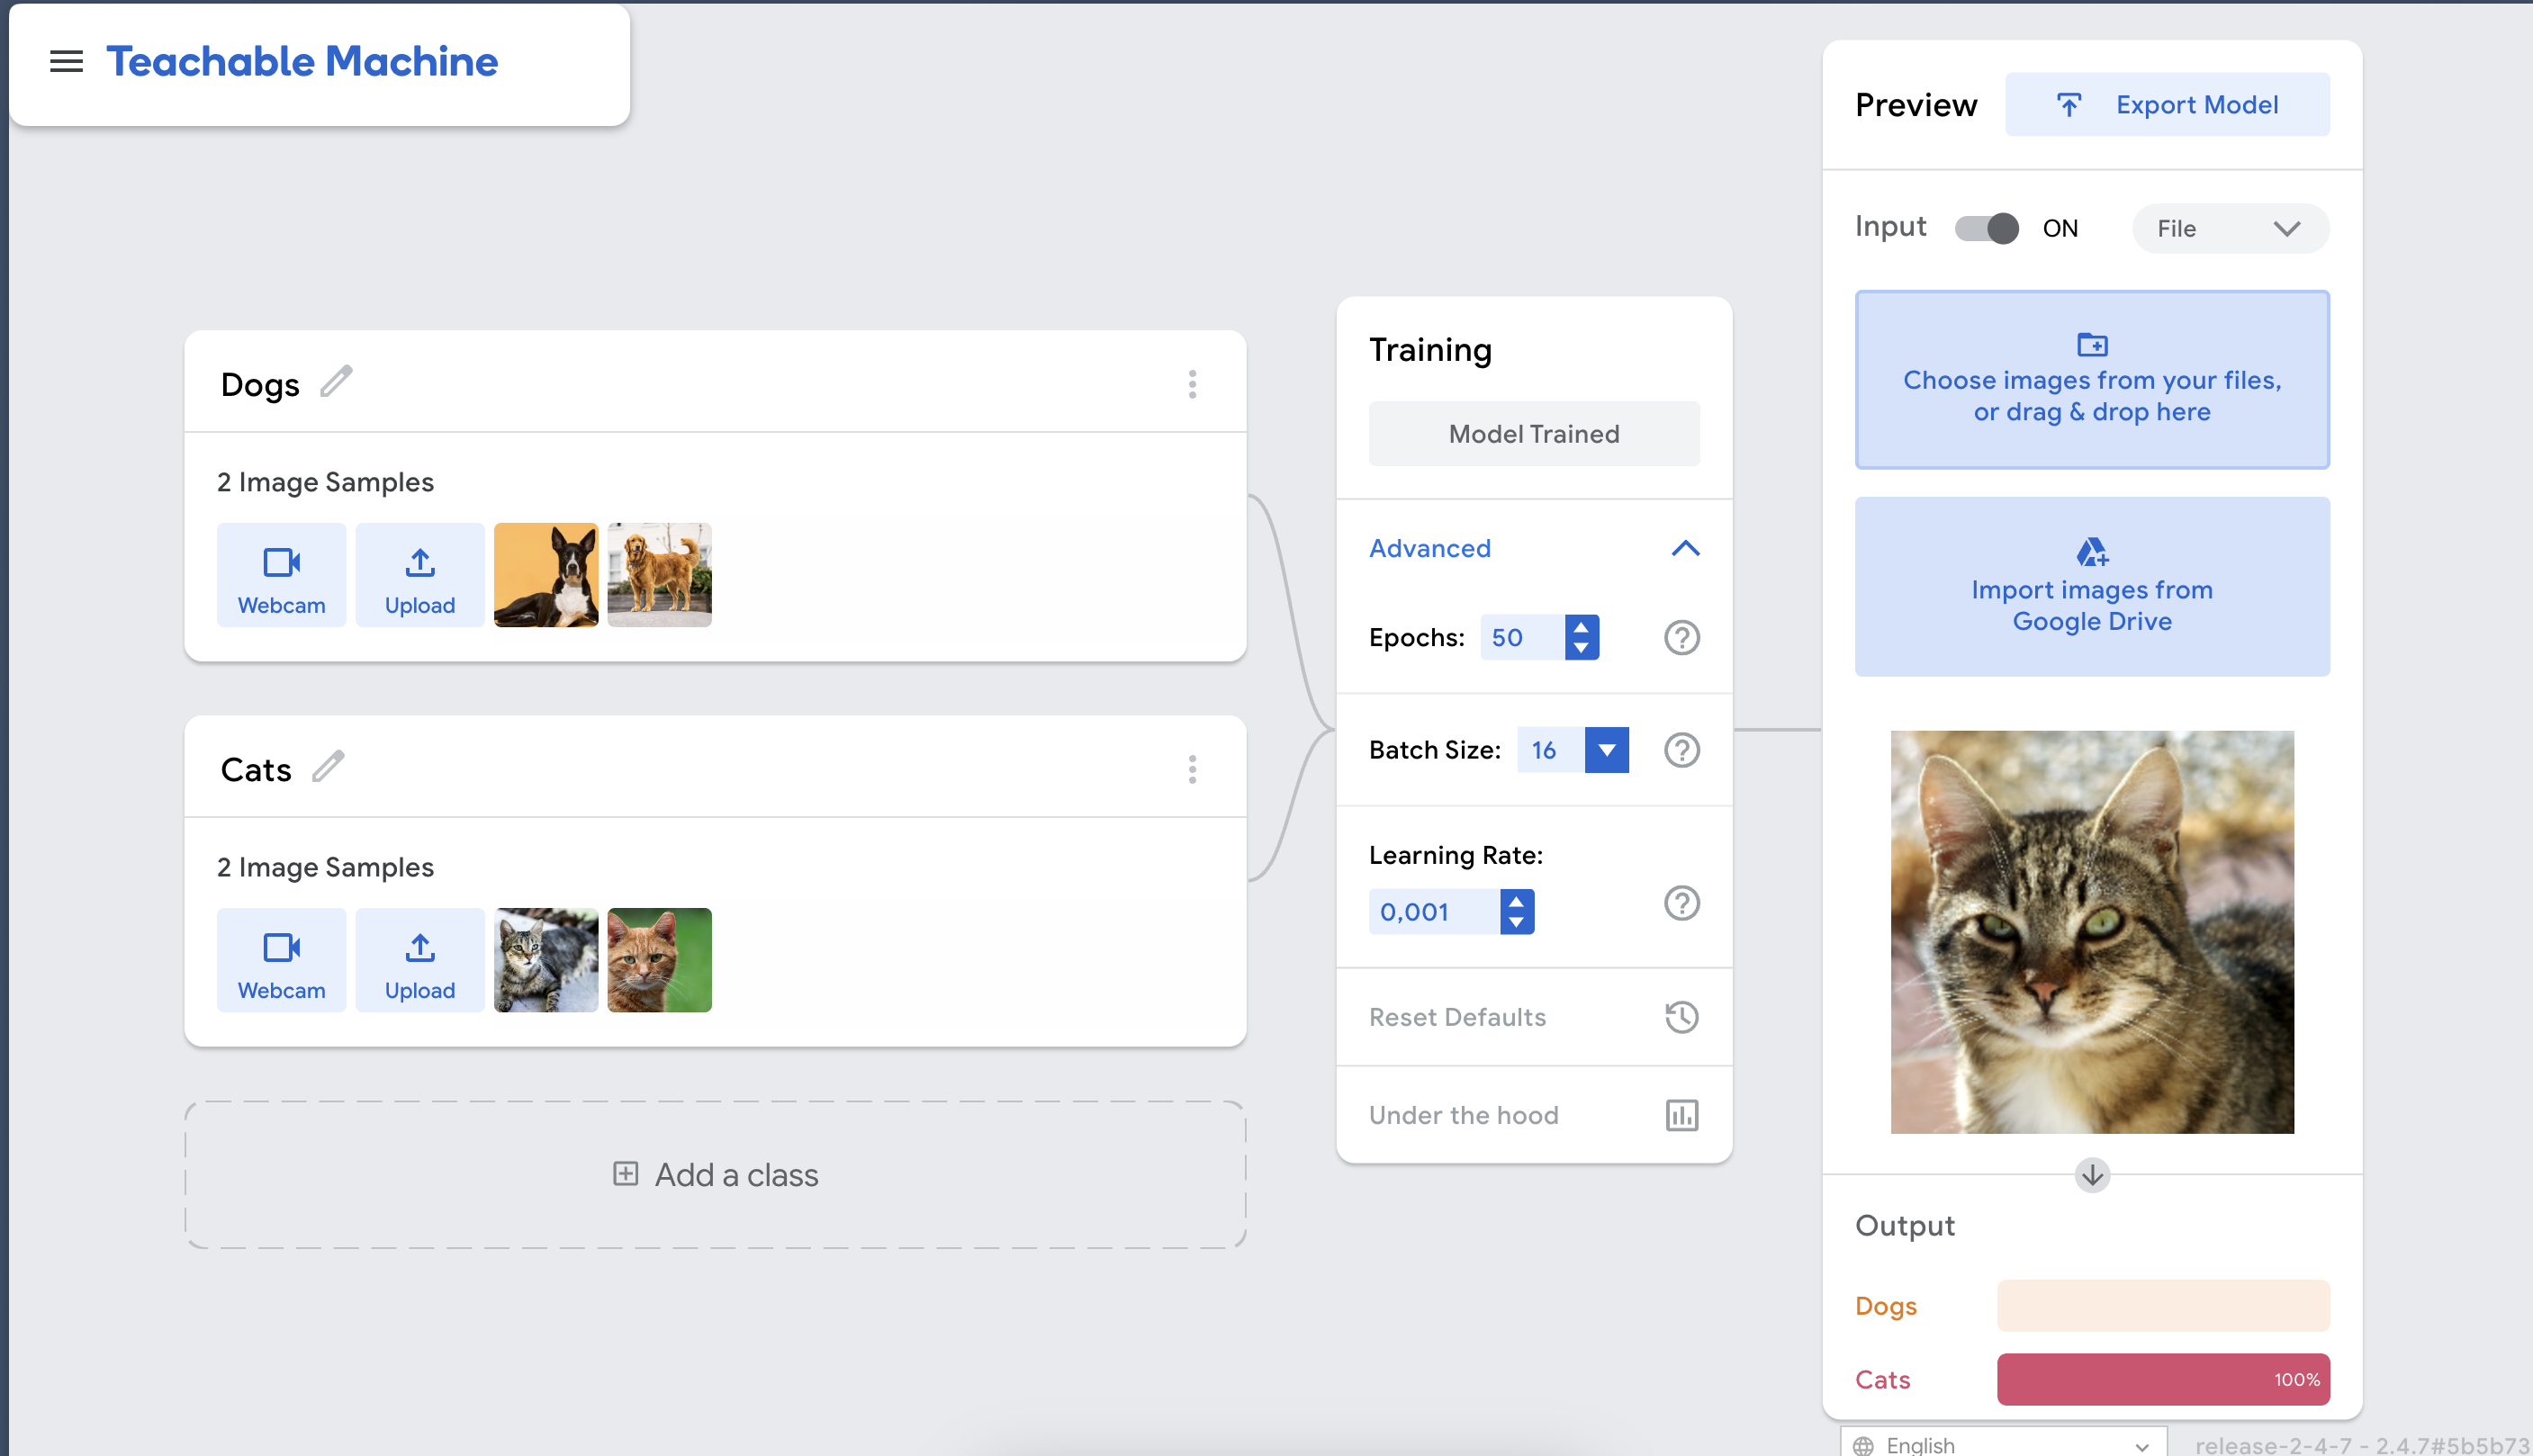
\includegraphics[width=\textwidth,keepaspectratio]{images/TeachableMachineExample.png}
    \caption{Usage of AI model in Teachable Machine website}
    \label{fig:appendix_image2}
\end{figure}



\end{document}
